\section{Results}
\label{sec:results}

\subsection{What changes query relevance}
\label{sec:main-findings}

Figure~\ref{fig:decomposition} sets the comparisons of Section~\ref{sec:decomposition-logic} side by side. Relation status matters little on average: superseded relevance exceeds other-attribute relevance by 0.314 nats (95\% CI [0.147, 0.482]) in Qwen and by 0.004 [−0.104, 0.118] in Gemma. Construction matters much more, with entity-mention relevance above superseded relevance by 3.504 [3.198, 3.806] and 2.589 [2.361, 2.829] nats. Mention order decides the sign for never-assigned values. Reversing the order lowers early-unassigned relevance by 6.578 [6.356, 6.789] nats in Qwen and 4.970 [4.700, 5.257] in Gemma, taking it from positive to negative, while the same reversal moves superseded relevance by only 0.340 [0.218, 0.470] and 0.032 [−0.101, 0.168]. For entity mentions the aligned-minus-reversed difference is large and has opposite signs in the two models: −1.969 [−2.344, −1.604] in Qwen and +1.810 [1.580, 2.058] in Gemma. In Experiment 2, adding \lit{Previously} lowers relevance by between 0.652 and 1.734 nats in each construction and model. Every change to how or where a value is mentioned moves $R$ more than switching the attribute it was assigned to, but only some of these effects point the same way in both models.

\begin{figure}[t]
\begin{center}
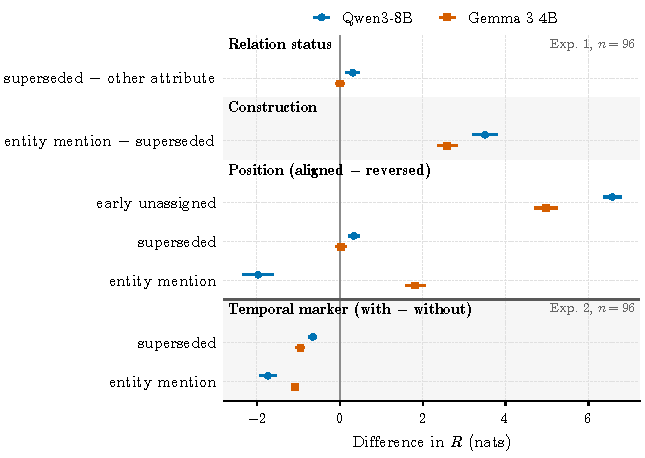
\includegraphics[width=0.68\linewidth]{figures/decomposition.pdf}
\end{center}
\caption{What changes query relevance. Every row is a difference in $R$ (nats) between two prompt variants, with 95\% history-bootstrap intervals. Relation status: superseded minus other attribute. Construction: entity mention minus superseded. Position: $R$ under aligned minus $R$ under reversed order, paired within history. Marker: $R$ with minus without \lit{Previously}, within each construction. Rows above the dark line come from Experiment 1 (96 histories); rows below it from Experiment 2 (96 histories, one entity pair and one attribute). Estimates are computed from the sealed analyses by \lit{scripts/fig\_decomposition.py}.}
\label{fig:decomposition}
\end{figure}

Table~\ref{tab:main} and Figure~\ref{fig:construction-order} give $R$ for every construction and order group. The live control shows the scale of a fully relevant edit: 32.598 nats in Qwen and 39.355 in Gemma. Superseded and other-attribute relevance are positive and similar in both order groups. Entity-mention relevance is the largest among the non-live constructions in both order groups. Unassigned relevance is near zero overall but large and of opposite sign in the two order groups.

\begin{table}[t]
\caption{Query relevance $R$ (nats) by construction and order group in Experiment 1, with 95\% history-bootstrap intervals over 96 histories. The live control has one assignment block, so it has no order split.}
\label{tab:main}
\begin{center}
\small
\begin{tabular}{@{}llrrr@{}}
\toprule
Model & Construction & Overall $R$ & Aligned $R$ & Reversed $R$ \\
\midrule
Qwen3-8B & Live & 32.598 [31.258, 33.967] & — & — \\
Qwen3-8B & Superseded & 1.974 [1.840, 2.109] & 2.144 [1.995, 2.301] & 1.804 [1.660, 1.947] \\
Qwen3-8B & Other attribute & 1.660 [1.488, 1.835] & 1.679 [1.527, 1.835] & 1.641 [1.422, 1.863] \\
Qwen3-8B & Entity mention & 5.478 [5.128, 5.825] & 4.493 [4.235, 4.770] & 6.463 [5.971, 6.940] \\
Qwen3-8B & Early unassigned & −0.037 [−0.203, 0.121] & 3.252 [3.046, 3.455] & −3.327 [−3.518, −3.150] \\
Qwen3-8B & Late unassigned & 0.001 [−0.208, 0.211] & 3.187 [2.948, 3.442] & −3.184 [−3.433, −2.945] \\
\midrule
Gemma 3 4B & Live & 39.355 [38.303, 40.415] & — & — \\
Gemma 3 4B & Superseded & 1.688 [1.568, 1.817] & 1.703 [1.574, 1.841] & 1.672 [1.529, 1.831] \\
Gemma 3 4B & Other attribute & 1.683 [1.541, 1.832] & 1.763 [1.598, 1.932] & 1.603 [1.453, 1.771] \\
Gemma 3 4B & Entity mention & 4.277 [4.029, 4.545] & 5.181 [4.884, 5.496] & 3.372 [3.131, 3.633] \\
Gemma 3 4B & Early unassigned & 0.113 [−0.023, 0.245] & 2.598 [2.395, 2.798] & −2.372 [−2.567, −2.178] \\
Gemma 3 4B & Late unassigned & 0.125 [−0.055, 0.305] & 3.445 [3.202, 3.696] & −3.194 [−3.447, −2.945] \\
\bottomrule
\end{tabular}
\end{center}
\end{table}

\begin{figure}[t]
\begin{center}
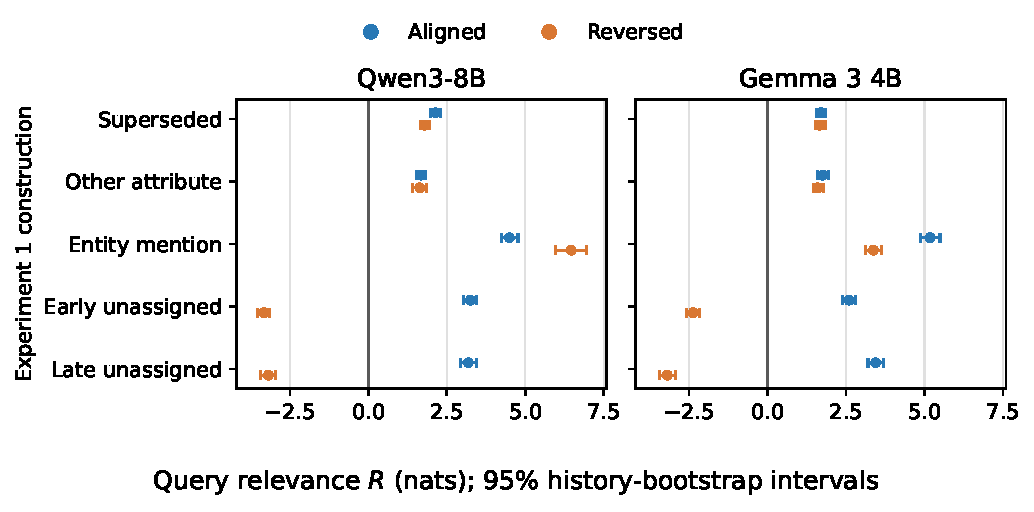
\includegraphics[width=0.98\linewidth]{figures/construction_by_order.pdf}
\end{center}
\caption{Query relevance $R$ (nats) for the five non-live constructions of Experiment 1, by order group and model. Points are means over 96 histories; intervals are 95\% history-bootstrap intervals. Live is omitted from the shared scale (Table~\ref{tab:main}). Paired order differences are in Table~\ref{tab:b-paired-r}.}
\label{fig:construction-order}
\end{figure}

These score changes coexist with correct rankings. In the superseded construction both models ranked the current value strictly first in all 1,536 baseline and all 1,536 edited prompts, with mean current-minus-earlier margins of 21.734 nats (Qwen) and 23.854 (Gemma). The edits changed source and donor scores that both had low absolute mass: Qwen's mean superseded source score fell from −22.271 to −23.881 while the donor score rose from −23.618 to −22.120 (Appendix~\ref{app:score-changes}). These changes do not imply that probability moves from one candidate to the other, or a matching change in generated answers.

\subsection{Relation status and construction}
\label{sec:relation}

Superseded minus other attribute is the study's closest estimate of what being an obsolete value of the queried attribute adds (Table~\ref{tab:frozen}; Section~\ref{sec:decomposition-logic} explains why it cannot separate the two properties involved). On average it adds 0.314 nats in Qwen, about a sixth of superseded relevance, and 0.004 in Gemma. The Qwen average masks heterogeneity: across target attributes it ranges from −0.570 for \lit{code} to 0.876 for \lit{color} (Table~\ref{tab:b-attr-other}); Gemma's attribute-specific intervals all include zero, which is not evidence of equivalence. Relation status is therefore small on average relative to construction, not uniformly negligible, and a follow-up shows that in Qwen the average combines two opposing effects (Section~\ref{sec:followups}).

Mentioning the earlier value in a note about the entity, without assigning it, produces more relevance than the superseded assignment in both models: superseded minus entity mention is −3.504 nats in Qwen and −2.589 in Gemma, and the sign holds for every target attribute (Table~\ref{tab:b-attr-entity}). The two constructions differ in predicate, syntax, name--value distance, and the presence of \lit{Previously}; Experiment 2 removes the marker difference (Section~\ref{sec:marker-results}) and a follow-up varies distance (Section~\ref{sec:followups}).

\begin{table}[t]
\caption{Superseded minus each control construction, $R_{\text{superseded}}-R_{\text{control}}$ (nats), with 95\% history-bootstrap intervals over 96 histories. Because early-unassigned $R$ is near zero after averaging over orders (Section~\ref{sec:order}), the last contrast is close to superseded $R$ itself. Order-stratified versions are in Table~\ref{tab:b-order}.}
\label{tab:frozen}
\begin{center}
\small
\begin{tabular}{@{}llrr@{}}
\toprule
Control & Isolates & Qwen3-8B & Gemma 3 4B \\
\midrule
Other attribute & relation status & 0.314 [0.147, 0.482] & 0.004 [−0.104, 0.118] \\
Entity mention & construction & −3.504 [−3.806, −3.198] & −2.589 [−2.829, −2.361] \\
Early unassigned & none: order-averaged control near zero & 2.011 [1.855, 2.170] & 1.575 [1.440, 1.719] \\
\bottomrule
\end{tabular}
\end{center}
\end{table}

These three contrasts were the test of our original hypothesis, which predicted that superseded relevance would exceed all three controls, each with a lower 95\% bound above zero, both overall and under reversed order. The prediction fails in both models, because the entity-mention contrast is negative overall and under reversed order (Table~\ref{tab:b-order}).

\subsection{Mention order}
\label{sec:order}

When no sentence links a value to an entity, the models link them by position. Under aligned order the first unassigned value sits in the same slot as the entity listed first in the current block, and an edit to it is more relevant to that entity's query; under reversed order the same value lines up with the other entity, and relevance turns negative (Table~\ref{tab:main}). The pattern holds for early and late unassigned mentions in both models, with paired order effects between 4.970 and 6.639 nats and positive in every one of the 96 histories (Table~\ref{tab:b-paired-r}). This is the behavior expected if values and entities are matched by ordinal position, consistent with the positional retrieval mechanism described by \citet{gurarieh2026mixing}; our data show the behavior, not the mechanism.

Explicit association does not remove order dependence, but it keeps relevance positive. Superseded relevance stays positive in both order groups (2.144 aligned and 1.804 reversed in Qwen; 1.703 and 1.672 in Gemma), with a small paired order effect. Entity-mention relevance also stays positive in both groups, but its paired order effect is large and model-specific: aligned order lowers it in Qwen (−1.969) and raises it in Gemma (+1.810). Averaging over orders hides the unassigned pattern entirely: overall unassigned relevance is near zero (−0.037 and 0.001 in Qwen; 0.113 and 0.125 in Gemma) not because the edit is ignored (an early unassigned edit shifts scores by 8.202 and 8.239 nats under the two queries in Qwen, and by 6.347 and 6.234 in Gemma) but because aligned and reversed effects cancel. The same cancellation makes superseded-minus-unassigned negative under aligned order and positive under reversed order (Figure~\ref{fig:order}, Appendix~\ref{app:exp1}).

\subsection{The explicit marker}
\label{sec:marker-results}

Experiment 2 adds or removes the prefix \lit{Previously,} with the rest of each prompt fixed (Table~\ref{tab:marker-templates}). Adding the marker lowers $R$ in both constructions and both models, with every within-construction interval below zero (Table~\ref{tab:marker}, Figure~\ref{fig:marker-effects}). In Qwen the reduction is larger for entity mentions: the marker-by-construction interaction is 1.082 [0.850, 1.308], positive in both order groups. In Gemma the two reductions are similar and the interaction, 0.125 [−0.012, 0.265], is not resolved; its order groups point in opposite directions. An earlier 24-history run of the same design gave the same pattern (Appendix~\ref{app:marker}). Relevance stays positive with the marker in every construction and order group, so the marker lowers the earlier value's influence without removing it. A lower score contrast is not evidence of active suppression.

Without the marker, entity-mention relevance still exceeds superseded relevance: by 3.059 [2.758, 3.370] nats in Qwen and 0.908 [0.783, 1.034] in Gemma, paired within history. The gap depends on order, however. In Gemma's reversed-order cell the difference is not resolved (entity minus superseded −0.175 [−0.357, 0.011]), and the marker leaves Gemma's gap almost unchanged (0.782 [0.673, 0.894] with the marker). An exploratory Phi-4-mini run on the earlier 24-history dataset showed yet another pattern, with the marker lowering superseded relevance (−1.355 [−1.561, −1.138]) but not entity-mention relevance (0.145 [−0.018, 0.310]; Appendix~\ref{app:marker}).

\begin{table}[t]
\caption{The four historical-line templates of Experiment 2, shown for Nora. Each prompt has two such lines, one per entity, followed by the current-state block and query of Experiment 1.}
\label{tab:marker-templates}
\begin{center}
\small
\begin{tabular}{@{}l>{\raggedright\arraybackslash}p{0.33\linewidth}>{\raggedright\arraybackslash}p{0.40\linewidth}@{}}
\toprule
Construction & Marker absent & Marker present \\
\midrule
Superseded & \lit{Nora's badge was amber.} & \lit{Previously, Nora's badge was amber.} \\
Entity mention & \lit{Nora mentioned amber in an unrelated note.} & \lit{Previously, Nora mentioned amber in an unrelated note.} \\
\bottomrule
\end{tabular}
\end{center}
\end{table}

\begin{table}[t]
\caption{Marker effects, $R_{\text{present}}-R_{\text{absent}}$, and the marker-by-construction interaction (superseded minus entity-mention marker effect) in Experiment 2, in nats, with 95\% history-bootstrap intervals over 96 histories. The underlying $R$ values, their source/donor components, and the earlier 24-history run are in Appendix~\ref{app:marker}.}
\label{tab:marker}
\begin{center}
\small
\begin{tabular}{@{}llrrr@{}}
\toprule
Model & Order & Superseded & Entity mention & Interaction \\
\midrule
Qwen3-8B & All & −0.652 [−0.748, −0.560] & −1.734 [−1.934, −1.536] & 1.082 [0.850, 1.308] \\
Qwen3-8B & Aligned & −0.366 [−0.484, −0.243] & −1.000 [−1.164, −0.834] & 0.635 [0.427, 0.841] \\
Qwen3-8B & Reversed & −0.938 [−1.071, −0.804] & −2.469 [−2.746, −2.189] & 1.530 [1.208, 1.847] \\
\midrule
Gemma 3 4B & All & −0.950 [−1.062, −0.841] & −1.075 [−1.166, −0.986] & 0.125 [−0.012, 0.265] \\
Gemma 3 4B & Aligned & −0.963 [−1.100, −0.834] & −1.445 [−1.566, −1.326] & 0.482 [0.307, 0.655] \\
Gemma 3 4B & Reversed & −0.937 [−1.112, −0.767] & −0.705 [−0.833, −0.580] & −0.232 [−0.436, −0.027] \\
\bottomrule
\end{tabular}
\end{center}
\end{table}

\begin{figure}[t]
\begin{center}
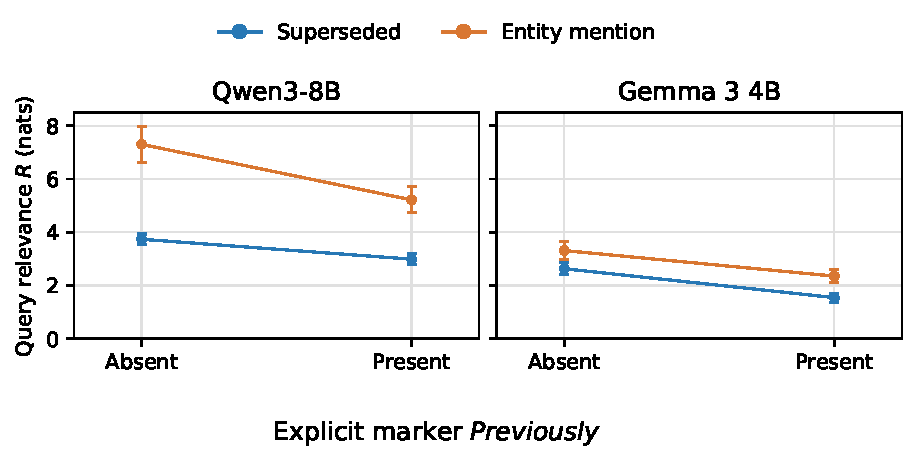
\includegraphics[width=0.78\linewidth]{figures/marker_by_construction.pdf}
\end{center}
\caption{Query relevance in Experiment 2 by marker and construction, averaged over orders. Points are means over 96 histories; intervals are marginal 95\% history-bootstrap intervals. Paired marker effects and the interaction, rather than overlap of marginal intervals, are in Table~\ref{tab:marker}.}
\label{fig:marker-effects}
\end{figure}

\subsection{Follow-up experiments}
\label{sec:followups}

\paragraph{Relation status splits into two opposing effects in Qwen.} With prompt length and layout matched, having been the queried attribute raised relevance (superseded minus updated other attribute: 0.740 [0.661, 0.818] nats in Qwen, 0.148 [0.038, 0.261] in Gemma), while being contradicted by an update lowered it in Qwen (updated minus static other attribute: −0.289 [−0.363, −0.215]) but not detectably in Gemma (−0.028 [−0.137, 0.076]; Table~\ref{tab:update}). In Qwen the two effects partly cancel, which is why the joint contrast of Experiment 1 was small; the recorded prediction of the discount account holds for Qwen and is unresolved for Gemma.

\begin{table}[t]
\caption{Updated-other-attribute follow-up: $R$ (nats) by construction and the two contrasts it separates, with 95\% history-bootstrap intervals over 96 histories. All three constructions share a six-line layout.}
\label{tab:update}
\begin{center}
\small
\begin{tabular}{@{}lrr@{}}
\toprule
 & Qwen3-8B & Gemma 3 4B \\
\midrule
Superseded & 1.368 [1.282, 1.457] & 0.817 [0.713, 0.928] \\
Other attribute, updated & 0.628 [0.555, 0.700] & 0.669 [0.568, 0.770] \\
Other attribute, not updated & 0.917 [0.835, 1.003] & 0.697 [0.602, 0.802] \\
\midrule
Queried attribute (superseded $-$ updated) & 0.740 [0.661, 0.818] & 0.148 [0.038, 0.261] \\
Update (updated $-$ not updated) & −0.289 [−0.363, −0.215] & −0.028 [−0.137, 0.076] \\
Superseded $-$ not updated & 0.451 [0.376, 0.525] & 0.120 [0.027, 0.209] \\
\bottomrule
\end{tabular}
\end{center}
\end{table}

\paragraph{Name--value distance does not explain the construction gap.} Moving the name next to the value raised superseded relevance in both models (near minus far: 0.500 [0.400, 0.599] in Qwen, 0.393 [0.288, 0.496] in Gemma) but did not raise entity-mention relevance: the near-minus-far difference was −0.370 [−0.498, −0.249] in Qwen and −0.027 [−0.110, 0.058] in Gemma (Table~\ref{tab:distance}). The recorded prediction, near above far in both constructions, therefore fails in both models; in Qwen's entity-mention construction the effect goes the other way. At matched near distance (one token between name and value in both constructions), entity mentions remain more influential than superseded assignments, by 1.293 [1.019, 1.571] nats in Qwen and 0.367 [0.234, 0.514] in Gemma, smaller than the far-condition gaps of 2.163 and 0.788. Proximity raises superseded relevance and so closes part of the gap, but not most of it in Qwen and not all of it in either model.

\begin{table}[t]
\caption{Name--value distance follow-up: $R$ (nats) by construction and distance, near-minus-far differences, and the entity-minus-superseded gap at each distance, with 95\% history-bootstrap intervals over 96 histories. Measured name--value gaps: one token in both near conditions; three (Qwen) or four (Gemma) tokens for superseded far; seven for entity-mention far.}
\label{tab:distance}
\begin{center}
\small
\begin{tabular}{@{}lrr@{}}
\toprule
 & Qwen3-8B & Gemma 3 4B \\
\midrule
Superseded, near & 2.685 [2.516, 2.861] & 2.005 [1.858, 2.135] \\
Superseded, far & 2.184 [2.030, 2.335] & 1.612 [1.492, 1.735] \\
Entity mention, near & 3.977 [3.684, 4.264] & 2.372 [2.245, 2.505] \\
Entity mention, far & 4.347 [4.043, 4.662] & 2.399 [2.261, 2.545] \\
\midrule
Superseded, near $-$ far & 0.500 [0.400, 0.599] & 0.393 [0.288, 0.496] \\
Entity mention, near $-$ far & −0.370 [−0.498, −0.249] & −0.027 [−0.110, 0.058] \\
\midrule
Entity $-$ superseded, near & 1.293 [1.019, 1.571] & 0.367 [0.234, 0.514] \\
Entity $-$ superseded, far & 2.163 [1.866, 2.459] & 0.788 [0.657, 0.922] \\
\bottomrule
\end{tabular}
\end{center}
\end{table}

Read across experiments, the construction gap shrinks as the two constructions are made more alike (Table~\ref{tab:gap}). In Experiment 1 only the superseded line carries \lit{Previously} and its value sits three or four tokens after the name, against one token in the entity-mention line; there the gap is 3.504 nats in Qwen and 2.589 in Gemma. With the marker on both lines it is 1.976 and 0.782 in Experiment 2, and with the marker on both lines and a one-token name--value distance in both it is 1.293 and 0.367 in the distance follow-up. The rows come from different stimulus sets (Experiment 2 uses one entity pair and one attribute), so they are matched comparisons rather than an additive decomposition. What remains at matched marker and distance, about 1.3 nats in Qwen and 0.4 in Gemma, is the part that predicate and framing would have to explain.

\begin{table}[t]
\caption{Entity-mention minus superseded relevance (nats) under increasingly matched conditions, with 95\% history-bootstrap intervals. ``Marker'' gives which construction carries \lit{Previously}; ``Gap'' gives the measured tokens between name and value (entity mention vs.\ superseded). Experiment 2 uses one entity pair and one attribute; the other rows use Experiment 1's allocation.}
\label{tab:gap}
\begin{center}
\small
\begin{tabular}{@{}llllrr@{}}
\toprule
Source & Marker & Gap & Histories & Qwen3-8B & Gemma 3 4B \\
\midrule
Experiment 1 & superseded only & 1 vs.\ 3--4 & 96 & 3.504 [3.198, 3.806] & 2.589 [2.361, 2.829] \\
Experiment 2 & neither & 1 vs.\ 3--4 & 96 & 3.059 [2.758, 3.370] & 0.908 [0.783, 1.034] \\
Experiment 2 & both & 1 vs.\ 3--4 & 96 & 1.976 [1.795, 2.169] & 0.782 [0.673, 0.894] \\
Distance follow-up, far & both & 7 vs.\ 3--4 & 96 & 2.163 [1.866, 2.459] & 0.788 [0.657, 0.922] \\
Distance follow-up, near & both & 1 vs.\ 1 & 96 & 1.293 [1.019, 1.571] & 0.367 [0.234, 0.514] \\
\bottomrule
\end{tabular}
\end{center}
\end{table}

\paragraph{More updates, more sensitivity in Qwen, while answers stay correct.} Both models answered every development prompt correctly at chain depths 3, 4, and 5 (384 generated answers per depth and model), so no depth fell in the 70--95\% window and, by the recorded rule, no generation confirmation was run. The candidate scores told a different story. On 96 histories per depth, Qwen's $R$ for the edited superseded value rose from 7.353 [6.972, 7.725] nats at depth 3 to 10.762 [10.303, 11.220] at depth 4 and 11.835 [11.424, 12.286] at depth 5; the depth-5-minus-depth-3 difference of 4.482 [3.915, 5.047] meets the recorded criterion. Gemma's $R$ stayed between 3.450 and 3.708 (depth 5 minus depth 3: 0.258 [−0.063, 0.557]). In Qwen, then, each additional update makes the scores more sensitive to the most recent superseded value even though no answer names it, a score-level counterpart of the interference that \citet{wang2025unable} observe in answers when updates accumulate (Appendix~\ref{app:followups}). Neither the chains nor the earlier distractor study (Appendix~\ref{app:harder}) lowered accuracy enough to test generated answers.

\paragraph{Below ceiling, generated answers follow the same pattern (exploratory).} OLMo-2's answers were correct for 2,950 of 3,072 superseded prompts but only 1,846 of 3,072 entity-mention prompts and 1,528 and 2,131 of the early- and late-unassigned prompts (Table~\ref{tab:olmo}). Its errors follow the pattern of the screened models' scores. Editing a value mentioned with the queried entity moved answers to the donor query-specifically (donor following 0.155 [0.124, 0.190]). Never-assigned values were named in about a tenth of answers and pulled them toward the entity in the matching position: early-unassigned donor following was 0.161 [0.122, 0.203] under aligned order and −0.164 [−0.214, −0.120] under reversed order, cancelling when orders are pooled. Superseded and other-attribute values almost never surfaced (0.9\% and 0.1\% of baseline answers to the edited entity's query named its earlier value), although the superseded edit still moved answers by a small, query-specific amount (0.008 [0.003, 0.014]). Where answers are not at ceiling, then, the earlier values that change scores are also the ones that change answers.

\begin{table}[t]
\caption{Exploratory generated-answer study in OLMo-2-7B-Instruct (outside the screened population) on the Experiment 1 confirmation set. Accuracy counts all 3,072 prompts per construction; donor following is the share of edited prompts answered with the donor under the edited entity's query minus under the other entity's query, with 95\% history-bootstrap intervals over 96 histories.}
\label{tab:olmo}
\begin{center}
\small
\begin{tabular}{@{}lrrrr@{}}
\toprule
Construction & Accuracy & Donor following & Aligned & Reversed \\
\midrule
Live & 2,970/3,072 & 0.948 [0.924, 0.969] & 0.948 & 0.948 \\
Superseded & 2,950/3,072 & 0.008 [0.003, 0.014] & 0.016 & 0.000 \\
Other attribute & 2,990/3,072 & 0.001 [0.000, 0.004] & 0.000 & 0.003 \\
Entity mention & 1,846/3,072 & 0.155 [0.124, 0.190] & 0.185 & 0.125 \\
Early unassigned & 1,528/3,072 & −0.001 [−0.022, 0.020] & 0.161 & −0.164 \\
Late unassigned & 2,131/3,072 & 0.005 [−0.022, 0.031] & 0.148 & −0.138 \\
\bottomrule
\end{tabular}
\end{center}
\end{table}

\paragraph{Additional models.} OLMo-2-7B-Instruct failed the competence screen, ranking the current value first on 426--452 of 576 prompts in the entity-mention and unassigned constructions (Appendix~\ref{app:followups}); by the protocol it is not part of the screened analysis. Qwen3-14B could not be loaded with int8 weights on the 16 GB GPU used for every other run. Phi-4-mini again failed the screen in entity mention (561/576); scored descriptively on the confirmation set, it resembled the screened models in construction and order, with entity-mention relevance above superseded relevance by 1.872 [1.664, 2.091] nats and order-averaged early-unassigned relevance near zero (0.027 [−0.069, 0.130]). Unlike them, its superseded relevance was slightly below other-attribute relevance (−0.152 [−0.266, −0.040]).
